\documentclass[a4paper, 12pt]{scrartcl}
\usepackage[utf8]{inputenc}
\usepackage{ngerman}
\usepackage{setspace}
\usepackage{geometry}
\usepackage[hidelinks]{hyperref}
\usepackage{xcolor,soul}
\usepackage{graphicx}

\geometry{a4paper, top=25mm, left=25mm, right=25mm, bottom=25mm}

\usepackage{xcolor}
\usepackage[normalem]{ulem}
\useunder{\uline}{\ulined}{}%
\DeclareUrlCommand{\bulurl}{\def\UrlFont{\ttfamily\color{blue}\ulined}}

\title{Seminar IT-Sicherheit}
\author{Kevin Seidel \\ Studiengang Informatik \\ Matrikelnummer: 943147}

\begin{document}
\pagenumbering{arabic}
\setcounter{page}{1}

Im folgenden Bericht werden die Ergebnisse von zwei verschiedenen Netzwerksimulationen dargelegt. Diese wurden nach der Vorgabe aus der {\color{blue}\uline{ \href{http://sys.cs.uos.de/lehre/rene/2013/aufgaben/PA_Blatt02.pdf}{Praktischen Aufgabe 2}}} durchgeführt. Dort wurden die zu verwendeten Durchsatzraten und die Netzwerktopologie festgelegt.
Dabei wereden zwei Szenarien betrachtet. In einem wird ein voll funktionsfähiges Netzwerk betrachtet, wohingegen im zweitem Szenario ein Netzwerk mit fehlerhafter Kabelverbindung betrachtet.
Das weitere Vorgehen dieses Berichtes orientiert sich am {\color{blue}\uline{ \href{http://sys.cs.uos.de/lehre/rene/2013/folien/Kap3-Messungen.pdf}{ Mesurement Cookbook}}}, welches in der Veranstaltung Rechnernetze vorgestellt wurde.

\section{Aufgabenstellung}
Die Aufgabe bestand darin zwei Netzwerksimulationen mit dem Simulationsprogramm ns-3 durchzuführen. Bei diesen Simulationen ging es um die Beobachtung der Datenraten bei einer TCP-Verbindung zwischen einem Server mit 5 Clients, welche über einen Router miteinander verbunden sind.
Die erste Simulation betrachtet ein funktionierendes Netzwerk ohne Fehler, wohingegen in der zweiten Simulation eine theoretische Beschädigung der Verbindung zwischen Router und Server simuliert wird. Diese Beschädigung bewirkt einen Paketverlust von 10% auf dieser Verbindung.
Dabei soll ein Vergleich zwischen den Datenraten der beiden Simulationen erstellt werden und die Ergebnisse analysiert werden.

\section{Netzwerkmodell}
Das zu simulierende Netzwerk besteht aus fünf Clients, einem Router und einem Server. 
Der Server hat eine Verbindung zum Router. Diese erlaubt einen maximalen Durchsatz von 1Mbit/s und hat eine Verzögerung von 20 ms.
Die fünf Clients verfügen ebenfalls über jeweils eine Verbindung zum Router, welche auch über einen Durchsatz von 1Mbit/s und eine Verzögerung von 20ms verfügen.
Alle Netzwerkgeräte verfügen über eine Drop Tail Queue, das heißt es werden erst Pakete verworfen, wenn die jeweilige Queue komplett gefüllt ist.
In der Simulation wird ein TCP-Stream vom Server zu jedem Client aufgebaut, welcher über den Router führt. Jeder Client versucht dabei einen Durchsatz von 1Mbit/s zu erreichen, wobei zwischen Router und Server maximal ein Durchsatz von 1Mbit/s realisiert werden kann, welcher sich auf die Clients aufteilt.

\begin{figure}[!htbp]
    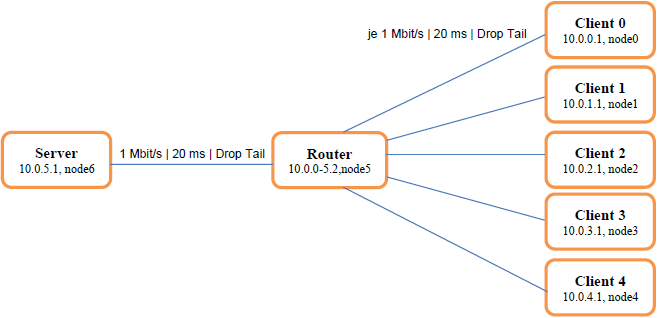
\includegraphics{Unbenannt.png}
  \caption{Netzwerktopologie}
  \label{Labelname}
\end{figure}


\section{Leistungsmetrik}
Da unsere Untersuchung sich auf das Verhalten des Durchsatzes ausrichtet, benötigen wir den Durchsatz pro Zeiteinheit über den Zeitraum der Simulation. 


\end{document}